\section{Modelling Security Properties with Automata}\label{SecMVA}

The automata that we use to express security properties are
called Property Automata (PA).  These
are extended finite state machines particularly suited for monitoring,
since transitions do not only depend on the automaton's state (\emph{i.e.},\
the current control point and a valuation for the automaton's
variables), but also on the state of the monitored program. 
% can
%depend on the state\footnote{The state of a PA
% consist of the current control point and values for the PA variables.}
% of the monitored program.
Transitions are labelled with guards, events and a list of
actions. Events specify the method whose entry and/or exit is being
monitored, with a distinction between normal and exceptional exits.
Guards describe the conditions under which a transition can be
applied. They depend on
\begin{inparaenum}[(\itshape i\upshape)]
\item the automaton state,
\item the state of the program that is being monitored, and
\item the argument of the method, in case the event is method entry;
the result of the method, in case the event is normal method exit; or
the exception with which the method returns, in case the event is
exceptional method exit.
\end{inparaenum}
Actions describe how the automaton state is updated by a transition.

Throughout, we assume that \(\CP\) and \(\Name\) are possibly infinite, but
countable non-empty sets of control points and names.  PA and
programs share the definitions of values, types and exceptions,
denoted \Val, \Type and \Excpt, respectively. These are defined by the
following grammar, where \(\BoolSet\) and \(\IntSet\) denote the
standard sets of booleans and integers, respectively\footnote{We will
use a PVS-like notation to declare abstract data types and records
(enclosed by \(\opr\) and \(\clr\)). Further, if \(x\) is a record
with field \textsf{y}, we use \(x.\mathsf{y}\) to access field
\textsf{y}, and \(x \opri\mathsf{y} := z\clri\) to denote the record
\(x\) with the field \textsf{y} updated to \(z\).}.
\[{\small
\begin{array}{rcl}
\Val & = & \B(b : \BoolSet) \mid \I(i : \IntSet) \mid \Null \mid
\R(i : \IntSet) \mid \One \mid \bot\\
\Type & = & \Bool \mid \Int \mid \Ref \mid \Void\\
\Excpt & = & \Throwable \mid \NullPointer \mid \JMLExc
\end{array}}
\]
The type \(\Void\), inhabited by \(\One\), models methods
without results; a reference can be \(\Null\) or contain a number
representing the location where the object is stored;
\(\bot\) is used to denote the outcome of an expression whose evaluation
is undefined (in Java this would typically result in an exception).

A PA consists of
\begin{inparaenum}[(\itshape i\upshape)]
\item a name,
\item a class name, to specify which class is being monitored,
\item a finite set of control points,
\item an initial control point,
\item a set of events, to specify which methods are being monitored,
\item a set of PA variable declarations, to describe
the internal state of the automaton,
\item a set of program variable declarations, to specify which
program variables will be inspected by the monitor, and
\item a set of transitions.
\end{inparaenum}
Transitions relate source and target control points. They are labelled
with events, where an event is a tuple of an event type (entry, exit
or exceptional exit) and a method name, a guard and a list of
actions. Each action assigns the result of an expression (containing
both program and PA variables) to a PA
variable. Notice that we only monitor classes here. This is often
the case in practice, because security-critical methods are often
static API methods. However, a more precise formalisation of Java's semantics
would allow to monitor objects as well. Formally, a PA is defined as follows.
% Figure~\ref{FigPAForm} shows the main components of the
% formal PA definition.
%\begin{figure}[t]

\vspace*{-1em}
\[{\small
\begin{array}{rcl}
\Decl & = \opr & \type : \Type, \name : \Name, \init : \Val
\clr \\
\EVENT & = \opr & \etype : (\entry \mid \exit \mid \excexit),
                 \mname : \Name \clr\\
\TRANS & = \opr & \scp, \tcp : \CP, \event : \EVENT, \action : (\opr \target : \Name, \expr : \Expr \clr)^*, \\
& &
\guard : \PAstate \times \Pstate \times (\Val \mid \Excpt) \rightarrow \BoolSet\clr\\
\PA & = \opr & \name, \clname : \Name, \cps : \setof{\CP},
            \init : \CP, \evs : \setof{\EVENT},\\
     &   &  \vdsA : \setof{\Decl}, \vdsP : \setof{\Decl},
            \trans : \setof{\TRANS} \clr
\end{array}}
\]
% \caption{Formal Definition of PA}\label{FigPAForm}
% \end{figure}

We require a PA to be \emph{deterministic}, \emph{i.e.}, for every source
control point and event there is always at most one guard that holds.
% Notice that it is not obvious how to transform a non-deterministic PA into
% a deterministic one, because the actions made by the overlapping transitions
% might differ.
% In theory it would be possible to relax this requirement by having a set of
% possible PA states (including values for the variables) but in practice this becomes clumsy.
A PA is \emph{total} if for any source control point and event,
there is always a guard that holds; otherwise it is
\emph{partial}. Every deterministic PA can be completed into a total
one (by function \complete): add a special control point
\halted, together with transitions for every control point and every event
to \halted, where the guard is the negation of the
disjunction of all other guards for this control point and event, and
in addition, add unconditional transitions from \halted to \halted
for every possible event.

% NOTE: these are not all the condition (for instance we are not saying that
% the expressions should not include Set statements or that the initial control
% point is in the set of control points and must not be halted.
A PA is \emph{wellformed} if:
% \footnote{We only formalise constraints that are necessary for our formalisation.}:
\begin{inparaenum}[(\itshape i\upshape)]
\item variable names are unique and are not reserved words,
\item guards do not have side-effects,
\item guards and actions only use declared variables, and
\item control points and events in transitions are declared.
\end{inparaenum}

The state of a PA consists of a current control point, and the store of
automaton variables (the program store is not part of the automaton state):
\({\small
\PAstate = \opr \cp : \CP, \stA : \Store \clr}
\). Given PA \(a\), the transition function \(\Delta_a\) specifies how
an automaton state \(\sigma_A\) is updated for a given program state
\(\sigma_P\), an event \(e\), and a value or exception \(v\) (where
\(\chooseop\) is the arbitrary choice operator, and \textsf{apply} is
a function that updates the automaton store according to a list of
actions in the obvious way).
\[{\small
\begin{array}{l}
\Delta_a  :  \PAstate \times \Pstate \times \EVENT \times (\Val \mid
\Excpt) \hookrightarrow
\PAstate\\
\Delta_a(\sigma_A, \sigma_P, e, v) = \\
\quad
\begin{array}[t]{l}
\mathsf{let\ }t = \chooseop(\{t\in \trans(a)\mid
  \begin{array}[t]{l}
     t.\scp = \sigma_A.\cp \wedge t.\event = e \wedge \\
     t.\guard(\sigma_A.\stA, \sigma_P.\fvs.\st, v)\}) \mathsf{\ in}
  \end{array}\\
\quad \opri \cp := t.\tcp, \stA := \mathsf{apply}(t.\action,
\sigma_A.\stA, \sigma_P.\fvs.\st) \clri
\end{array}

\end{array}}
\]
In a total PA $a$, the transition function \(\Delta_a\) is total.
A partial automaton gets stuck on a certain input if and only if the
completed PA reaches the state \halted.
\vspace*{-.5em}
\begin{equation}\label{PAcompletionProp}
\Delta_a(\sigma_A, \sigma_P, e, v) = \perp \Leftrightarrow
\Delta_{\complete(a)}(\sigma_A, \sigma_P, e, v).\cp = \halted
\end{equation}


\paragraph{Example}
The property specified in Fig.~\ref{FigExample} is encoded by the
following PA\footnote{Where we leave the default guard
\(\lambda(\sigma_A, \sigma_P, v). \ttt\) and  empty action
\(\actskip\) implicit.}, while Fig.~\ref{FigCompletePA} shows the
completed PA (where new transitions are dashed).

\vspace*{-1em}
{\small{
\hspace{-0.3em}
\begin{longtable}[t]{lll}
\(\opri\) &
\multicolumn{2}{l}
  {\(\name := \textrm{LimitSMS}, \clname := \texttt{Messaging},
  \cps := \{s_1, s_2\},
  \init := s_1,\)}\\
& \multicolumn{2}{l}{
  \(\evs :=
    \begin{array}[t]{l}
     \{ \opri \etype := e,
        \mname := \texttt{sendSMS} \clri
        \mid e \in \{ \entry, \exit, \excexit \} \} \:\cup \\
     \{ \opri \etype := \exit, \mname := \texttt{reset} \clri\},
    \end{array}\)} \\
& \multicolumn{2}{l}{
    \(\vdsA := \{\opri \name := n, \type := \Int, \init := 0 \clri\},
    \vdsP := \emptyset,\)}\\
& \(\trans := \{ \) &
       \(\opri
        \begin{array}[t]{l}
           \scp := s_1, \tcp := s_2,
           \guard := \lambda(\sigma_A, \sigma_P, v). n(\sigma_A) < N,\\
           \event := \opri \etype := \entry,
                     \mname := \texttt{sendSMS} \clri \clri,
        \end{array}\)\\
&&
     \(\opri
        \begin{array}[t]{l}
           \scp := s_2, \tcp := s_1,
           \action := [\opri \target := n, \expr := n + 1 \clri]\\
           \event := \opri \etype := \exit,
                     \mname := \texttt{sendSMS} \clri \clri,
        \end{array}\)\\
&&
     \(\opri
        \begin{array}[t]{l}
           \scp := s_2, \tcp := s_1, \\
           \event := \opri \etype := \excexit,
           \mname := \texttt{sendSMS} \clri \clri,
        \end{array}\)\\
&&
     \(\opri
        \begin{array}[t]{l}
           \scp := s_1, \tcp := s_1,
           \action := [\opri \target := n, \expr := 0 \clri], \\
           \event := \opri \etype := \exit, \mname := \texttt{reset}
           \clri \clri \} \clri
        \end{array}\)
\end{longtable}
}}

% \small{
% \hspace{-0.3em}
% \begin{longtable}[t]{l}
% \opri
% \begin{longtable}[t]{l}
% \(\name := \textrm{LimitSMS}, \clname := \texttt{Messaging},
% \cps := \{s_1, s_2\},
% \init := s_1,\)\\
% \(\evs :=
% \begin{array}[t]{l}
% \{ \opri \etype := e, \mname := \texttt{sendSMS} \clri \mid e \in \{ \entry,
% \exit, \excexit \} \} \:\cup \\
% \{ \opri \etype := \exit, \mname := \texttt{reset} \clri\},
% \end{array}\)
% \\
% \(\vdsA := \{\opri \name := n, \type := \Int, \init := 0 \clri\},
% \vdsP := \emptyset,\)\\
% \(\trans := \{
% \begin{array}[t]{l}
% \opri
%  \begin{array}[t]{l}
% \scp := s_1, \tcp := s_2, \guard := \lambda(\sigma_A, \sigma_P, v). n(\sigma_A) < N,\\
%              \event := \opri \etype := \entry,
%                              \mname := \texttt{sendSMS} \clri \clri,
% \end{array}\)\\
% \(\opri
%  \begin{array}[t]{l}
% \scp := s_2, \tcp := s_1, \action := [\opri \target := n, \expr := n + 1 \clri]\\
%              \event := \opri \etype := \exit,
%                              \mname := \texttt{sendSMS} \clri \clri,
% \end{array}\\
% \opri
%  \begin{array}[t]{l}
% \scp := s_2, \tcp := s_1, \\
%              \event := \opri \etype := \excexit,
%                              \mname := \texttt{sendSMS} \clri, \clri,
% \end{array}\\
% \opri
% \begin{array}[t]{l}
% \scp := s_1, \tcp := s_1, \action := [\opri \target := n, \expr := 0 \clri] \\
%              \event := \opri \etype := \exit, \mname := \texttt{reset} \clri \clri
% \} \clri
% \end{array}
% \end{array}\)
% \end{longtable}\\
% \end{longtable}
% }

\begin{figure}[h]

\psfrag{s1}{\tiny{\(s_1\)}}
\psfrag{s2}{\tiny{\(s_2\)}}
\psfrag{exit(sendSMS)?true -> n := n + 1;}
{\begin{tabular}{l}
\tiny{\exit(\texttt{SendSMS})?\ttt}\vspace*{-.8em}\\
\tiny{\(\rightarrow\)\texttt{n := n + 1};}
\end{tabular}}
\psfrag{exitE(sendSMS)?true -> ;}
{\begin{tabular}{l}
\tiny{\excexit(\texttt{sendSMS})?\ttt \(\rightarrow\)}%\vspace*{-.8em}\\
\tiny{\actskip;}
\end{tabular}}
\psfrag{exit(reset)?true -> n := 0;}
{\begin{tabular}{l}
\tiny{\exit(\texttt{reset})?\ttt \(\rightarrow\)}\vspace*{-.8em} \\
\tiny{\texttt{n :=} 0;}
\end{tabular}}
\psfrag{entry(sendSMS)? n<N -> ;}
{\begin{tabular}{l}
\tiny{\entry(\texttt{sendSMS})? \texttt{n} \(<\) \texttt{N} \(\rightarrow\)} %\vspace*{-.8em} \\
\tiny{\actskip;}
\end{tabular}}
\psfrag{entry(sendSMS)?true -> ;}
{\tiny{\entry(\texttt{sendSMS})?\ttt \(\rightarrow\)\actskip}}
\psfrag{exit(reset)?true -> ;}
{\tiny{\exit(\texttt{reset})?\ttt \(\rightarrow\)\actskip}}
\psfrag{exit(sendSMS)?true -> ;}
{\tiny{\exit(\texttt{sendSMS})?\ttt \(\rightarrow\)\actskip}}
\psfrag{exitE(sendSMS)?true -> ;}
{\tiny{\excexit(\texttt{sendSMS})?\ttt \(\rightarrow\)\actskip}}
\psfrag{entry(sendSMS)?n >= N -> ;}
{\tiny{\entry(\texttt{sendSMS})?\texttt{n} \(\geq\) \texttt{N}
\(\rightarrow\)\actskip}}
\psfrag{halted}{\tiny{\halted}}

\begin{center}
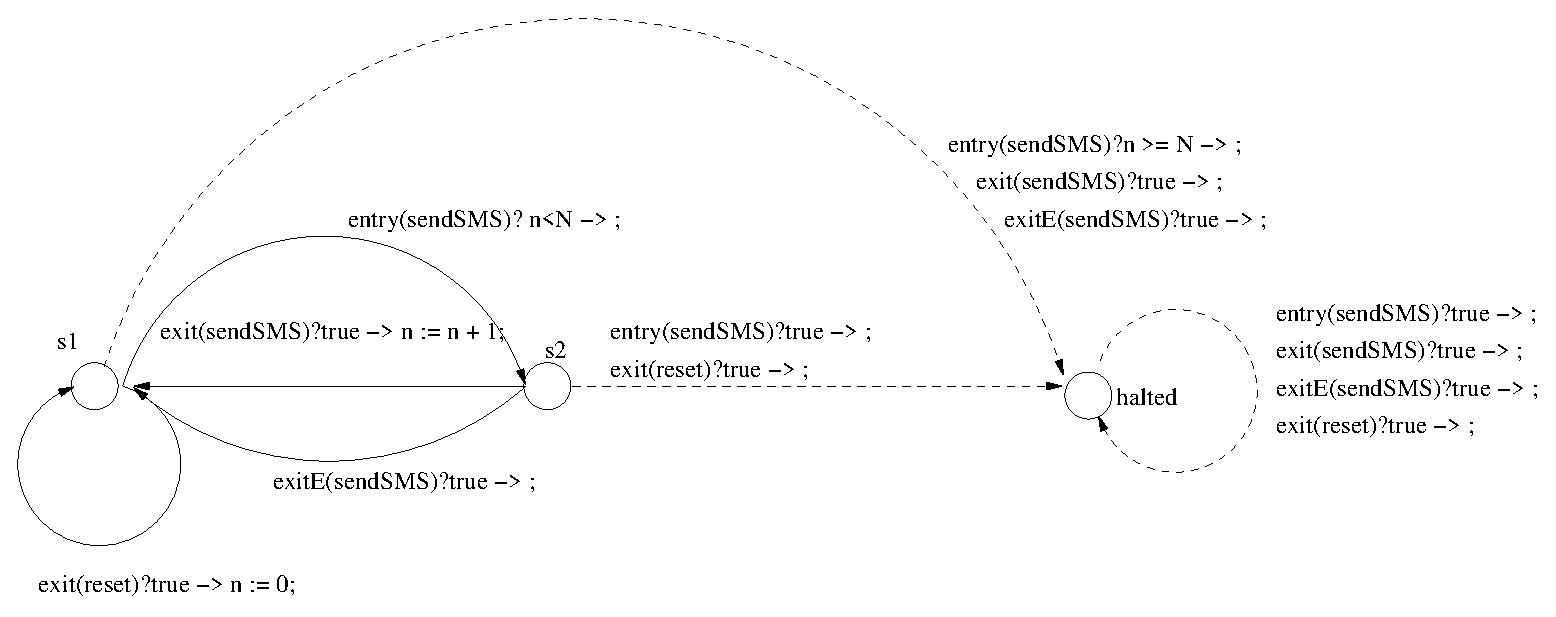
\epsfig{file=complete.eps, width=7cm}
\end{center}
\caption{Automaton of Fig.~\ref{FigExample}, after completion}\label{FigCompletePA}
\end{figure}
